\documentclass[conference]{IEEEtran}
% \IEEEoverridecommandlockouts
% The preceding line is only needed to identify funding in the first footnote. If that is unneeded, please comment it out.
\usepackage{cite}
\usepackage{amsmath,amssymb,amsfonts}
\usepackage{algorithmic}
\usepackage{graphicx}
\usepackage{textcomp}
\usepackage{xcolor}
\def\BibTeX{{\rm B\kern-.05em{\sc i\kern-.025em b}\kern-.08em
    T\kern-.1667em\lower.7ex\hbox{E}\kern-.125emX}}
\begin{document}

\bibliographystyle{IEEEtran}

\title{Applying ResNet and Inception Module Techniques for Skin Cancer Classification on Breast Histopathology Images Dataset with Convolutional Neural Networks\\
}

\author{\IEEEauthorblockN{1\textsuperscript{st} Pedro Almeida}
\IEEEauthorblockA{\textit{Department of Ocean \& Mechanical Engineering} \\
\textit{Florida Atlantic University}\\
Boca Raton, United States \\
palmeida2016@fau.edu}
}

\maketitle

\begin{abstract}
This document is a model and instructions for \LaTeX.
This and the IEEEtran.cls file define the components of your paper [title, text, heads, etc.]. *CRITICAL: Do Not Use Symbols, Special Characters, Footnotes, 
or Math in Paper Title or Abstract.
\end{abstract}

\begin{IEEEkeywords}
component, formatting, style, styling, insert
\end{IEEEkeywords}

\section{Introduction}
Over the past 40 years, the field of object detection in machine learning has made massive strides in classification and detection capabilities \cite{Fukushima1980}. In addition to the expected improvements stemming from larger datasets, deeper models, and more powerful machines, much of the advancement owes to new and improved network architectures and novel algorithms. The objective of this paper is to combine some of the novel techniques introduced in network architecture that widen a network without greatly increasing the computational cost of the model \cite{He2016, Szegedy2014}.

The objective of the report is to explore the combinations of these novel techniques through the Breast Histopathology Dataset \cite{Mooney2017}. The dataset contains 162 whole mount slide images of a breast cancer variant called Invasive Ductal Carcinoma scanned at forty-times magnification. As of 2019, breast cancer affects 1 in 8 women during their lifetime, registering roughly 268,600 new cases every year \cite{DeSantis2019}. Invasive Ductal Carcinoma, also known as Infiltrating Ductal Carcinoma, is the most common type breast cancer, accounting for 80\% of breast cancer diagnoses \cite{Sharma2010}. As is the case for most cancers, early detection accounts for most of successful treatments of the disease; as the cancer progresses to the later stages, the odds of spreading to nearby organs increases, thus furthering the risk of the death of the patient \cite{Milosevic2018}.



Each of the 162 samples in the dataset have been partitioned to create 277,524 50x50-pixel patches of which 198,738 are IDC negative and 78,786 are IDC positive. 

\section{Related Work}
Since the introduction of Convolutional Neural Networks (CNN), the model architecture off CNNs has remained largely static: a series of convolutional layers followed by optional normalization and pooling layers and finally one or more dense layers reducing to the output. This standard architecture and its variations have reigned dominant in accurately classifying objects in small and large datasets alike, from MNIST, CIFAR, ImageNet, MS-COCO, SVHN, and others. For larger datasets especially, the latest novel idea has been the introduction of deeper networks with dropout layers to correct for overfitting.

The tradeoff for adding more layers to a network is apparent in the time to train; as the model grows in size and increases the number of weights, the backwards propagation in updating the weights takes progressively longer, thus greatly adding to the required time to train. Furthermore, although the development of newer, more powerful machines and better parallelization and multi-processing techniques can somewhat mitigate the additional computational cost.
\section{Methods}
\subsection{ResNet Layer}
The first CNN idea applied in the model architecture employs residual learning within the convolution layers. As described by He \textit{et al.}, let us consider a residual layer within a neural network defined as:

\begin{equation}
y = \mathcal{F} \left(x,\{W_i\}\right) + x
\label{residual_layer_equation}
\end{equation}

In Eq. \ref{residual_layer_equation}, $x$ and $y$ are the input and output vectors of the layer respectively. The function $\mathcal{F} \left(x,\{W_i\}\right)$ represents the convoluntional mapping of inputs to outputs given a set of weights $W$ \cite{He2016}. For the example shown in Fig. \ref{ResNet Layer Model}, the input $x$ to the layer passes through 4 convolutional layers, which together constitute $\mathcal{F}(x)$ before the concatenation with the input $x$.

\begin{figure}
\centering
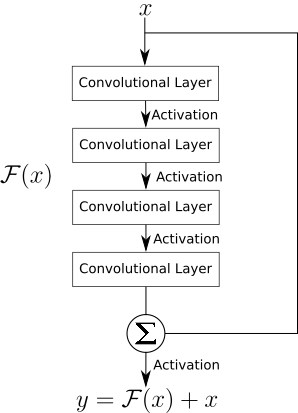
\includegraphics[scale=0.65]{figures/ResNet_Model.png}
\label{ResNet Layer Model}
\caption{Model of ResNet Layer with 4 Convolutions followed by concatenation.}
\end{figure}

\subsection{Inception Module Layer}
\subsection{Network Architecture}
\subsection{Data Augmentation}
\subsection{Training the Network}

\section{Results}

\section{Analysis and Discussion}

\section{Conclusions}

\section*{Acknowledgment}

\bibliography{citations}

\end{document}
